\documentclass[10pt,a4paper]{article}
\usepackage[margin=18mm]{geometry}
\usepackage[T1]{fontenc}
\usepackage{tgheros}
\renewcommand{\familydefault}{\sfdefault}
\usepackage{microtype,booktabs,tabularx,array,xcolor,tikz,qrcode}
\usepackage[hidelinks]{hyperref}
\usetikzlibrary{positioning,arrows.meta}
\definecolor{ink}{HTML}{151515}
\definecolor{muted}{HTML}{555555}
\definecolor{wash}{HTML}{F1F1F1}
\color{ink}
\pagestyle{empty}
\setlength{\parindent}{0pt}
\setlength{\parskip}{5pt}
\renewcommand{\arraystretch}{1.24}
\newcommand{\labelhead}[1]{{\small\bfseries #1}\par\vspace{2pt}}
\begin{document}
{\fontsize{28}{30}\selectfont\bfseries Aktina}\hfill{\small 4 October 2026}\par
\vspace{2mm}
{\Large Solar forecasting}\hfill{\small\color{muted}Technical summary}\par
\vspace{2mm}
Day-ahead solar forecasts for water-production planning.
\vspace{2mm}

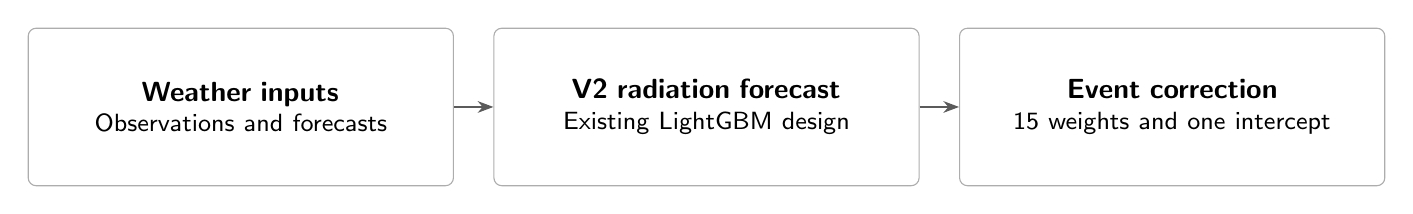
\begin{tikzpicture}[node distance=5mm,box/.style={draw=ink!35,rounded corners=1mm,minimum height=20mm,text width=48mm,align=center,inner sep=3mm},flow/.style={-{Stealth[length=2mm]},draw=ink!70}]
\node[box] (input) {\textbf{Weather inputs}\\[-1pt]{\small Observations and forecasts}};
\node[box,right=of input] (base) {\textbf{V2 radiation forecast}\\[-1pt]{\small Existing LightGBM design}};
\node[box,right=of base] (head) {\textbf{Event correction}\\[-1pt]{\small 15 weights and one intercept}};
\draw[flow] (input.east)--(base.west);
\draw[flow] (base.east)--(head.west);
\end{tikzpicture}

\vspace{2mm}
\labelhead{Measured result}
All methods use the same 3,566 hourly targets from 5 December 2025 to 3 May 2026. A positive event means observed radiation strictly above 600 W/m$^2$.

{\small
\begin{tabularx}{\linewidth}{@{}Xrrrrr@{}}
\toprule
Forecast & Precision & Recall & F1 & False alarms & Misses\\
\midrule
Previous day & 79.74\% & 79.74\% & 79.74\% & 62 & 62\\
Original v1 & 81.42\% & 78.76\% & 80.07\% & 55 & 65\\
Supplied v2 & 91.29\% & 85.62\% & 88.36\% & 25 & 44\\
Research 008 & 92.81\% & 88.56\% & 90.64\% & 21 & 35\\
\bfseries V2 + correction & \bfseries94.08\% & \bfseries88.24\% & \bfseries91.06\% & \bfseries17 & \bfseries36\\
\bottomrule
\end{tabularx}}

\textbf{Against supplied v2: eight more events found and eight fewer false alarms.} Against 008: four fewer false alarms, with one additional missed hour.

\vspace{2mm}
\begin{minipage}[t]{.475\linewidth}\raggedright
\labelhead{How it works}
The original v2 source is retained. Its nine-input design is refitted with early stopping inside training, then frozen. A small logistic correction reads its radiation estimate, weather-forecast disagreement, solar timing and four trailing 14-day error summaries.

The event call is $p>0.49$. Its threshold is chosen from earlier training predictions. The correction changes event decisions, not the radiation curve. The refit's MAE is 18.7007 W/m$^2$, versus 18.6973 for supplied v2.
\end{minipage}\hfill
\begin{minipage}[t]{.475\linewidth}\raggedright
\labelhead{How it was checked}
Expanding chronological folds and target-time purges keep future labels out of training. Past-error inputs use only observations resolved before each forecast origin. Saved coefficients, all hourly decisions and unsuccessful experiments are retained.

Independent replay reproduced the decisions and scores. Source hashes, fold membership and past-context invariance were checked. The approach adapts forecast stacking and statistical post-processing [1,2].
\end{minipage}

\vspace{3mm}
\labelhead{What the evidence supports}
This is an observed gain on reused historical validation. The paired-day 95\% interval for the F1 difference against 008 is $-1.61$ to $+2.62$ percentage points, including zero. It is not an established gain on unseen data. Targets are weather-derived, not local sensor readings. Archive issue-time availability is unverified. No curtailment recovery, plant performance or operating savings is established.

\vspace{3mm}
\hrule height .3pt
\vspace{3mm}
\begin{minipage}[c]{.77\linewidth}
\labelhead{Interactive demonstration}
\href{https://aktina-pafos-2026.vercel.app/forecast.html}{\textbf{aktina-pafos-2026.vercel.app/forecast.html}}\\
{\small Select a day, inspect an hour and compare forecasts.\\Historical predictions, not a live forecast feed.}

{\footnotesize\color{muted}\href{https://github.com/stefanosbordea/aktina/tree/stefanos-model/app/experiments/v2-019}{Reproducible method, source pins, fitted coefficients and independent audit.}}
\end{minipage}\hfill
\begin{minipage}[c]{.18\linewidth}\centering
\qrcode[height=24mm]{https://aktina-pafos-2026.vercel.app/forecast.html}
\end{minipage}

\vspace{3mm}
{\scriptsize\color{muted}
[1] D. H. Wolpert. \emph{Stacked generalization}. Neural Networks, 1992. \href{https://doi.org/10.1016/S0893-6080(05)80023-1}{doi:10.1016/S0893-6080(05)80023-1}.\par
[2] B. Schulz et al. \emph{Post-processing numerical weather prediction ensembles for probabilistic solar irradiance forecasting}. Solar Energy 220, 2021. \href{https://doi.org/10.1016/j.solener.2021.03.023}{doi:10.1016/j.solener.2021.03.023}.
}
\end{document}
